\documentclass[UTF8, 12pt]{article}

\usepackage{amsmath, amsfonts, amssymb, extarrows,enumerate,geometry}
\usepackage{tikz,pgfplots,xcolor}
\usepackage[bookmarks=true, colorlinks,allcolors=black]{hyperref}
\usetikzlibrary{patterns}

\geometry{papersize={12cm,12cm},left=0cm,right=0cm,top=0cm,bottom=0cm}


\begin{document}
\centering
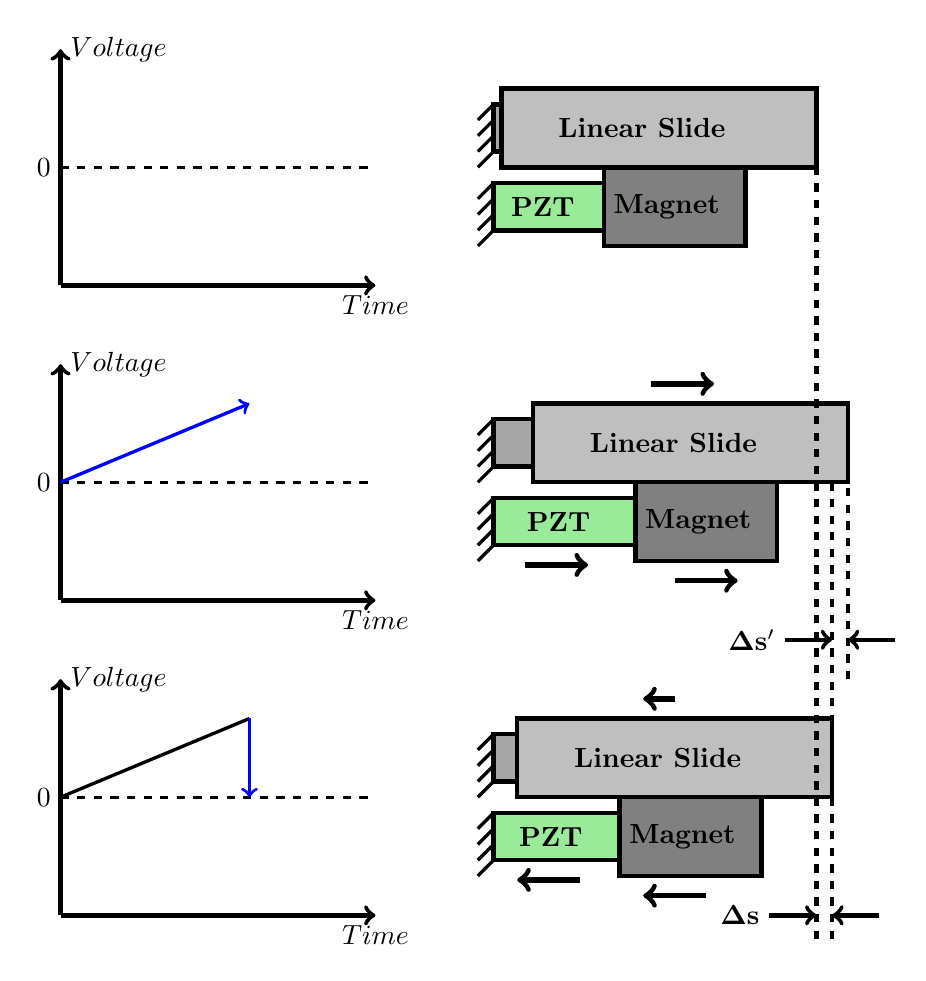
\begin{tikzpicture}
%	\draw[help lines, color=black!30, step=1cm,ultra thin](0,0)grid(10,12);
	
	\begin{scope}
		\draw [->,ultra thick, black](0,0)--(4,0);
		\draw [->,ultra thick, black](0,0)--(0,3);
		\node at (0,3)[right]{$Voltage$};
		\node at (4,0)[below]{$Time$};
		\draw [dashed,very thick,black](0,1.5)--(4,1.5);
		\node at (0,1.5)[left]{$0$};
		\draw [very thick,black](0,1.5)--(2.4,2.5);
		\draw [very thick,blue,->](2.4,2.5)--(2.4,1.5);
	\end{scope}
	
	\begin{scope}[shift={(0,4)}]
		\draw [->,ultra thick, black](0,0)--(4,0);
		\draw [->,ultra thick, black](0,0)--(0,3);
		\node at (0,3)[right]{$Voltage$};
		\node at (4,0)[below]{$Time$};
		\draw [dashed,very thick,black](0,1.5)--(4,1.5);
		\node at (0,1.5)[left]{$0$};
		\draw [very thick,blue,->](0,1.5)--(2.4,2.5);
	\end{scope}
	
	\begin{scope}[shift={(0,8)}]
		\draw [->,ultra thick, black](0,0)--(4,0);
		\draw [->,ultra thick, black](0,0)--(0,3);
		\node at (0,3)[right]{$Voltage$};
		\node at (4,0)[below]{$Time$};
		\draw [dashed,very thick,black](0,1.5)--(4,1.5);
		\node at (0,1.5)[left]{$0$};
	\end{scope}
	
	\begin{scope}[shift={(0.5,0.5)}]
		\begin{scope}
			\draw [black,very thick,shift={(0,-0.2)}](4.8,0.2)--(5,0.4);
			\draw [black,very thick](4.8,0.2)--(5,0.4);
			\draw [black,very thick,shift={(0,0.2)}](4.8,0.2)--(5,0.4);
			\draw [black,very thick,shift={(0,0.4)}](4.8,0.2)--(5,0.4);
		\end{scope}
		\begin{scope}[shift={(0,1)}]
			\draw [black,very thick,shift={(0,-0.2)}](4.8,0.2)--(5,0.4);
			\draw [black,very thick](4.8,0.2)--(5,0.4);
			\draw [black,very thick,shift={(0,0.2)}](4.8,0.2)--(5,0.4);
			\draw [black,very thick,shift={(0,0.4)}](4.8,0.2)--(5,0.4);
		\end{scope}
		\draw [fill=green!80!black!40,draw=black,ultra thick](5,0.2)rectangle(6.6,0.8);
		\draw [fill=gray,draw=black,ultra thick,shift={(0.1,0)}](6.5,0)rectangle(8.3,1);
		\draw [fill=gray!70,draw=black,ultra thick](5,1.2)rectangle(6.5,1.8);
		\draw [fill=gray!50,draw=black,ultra thick,shift={(0.1,0)}](5.2,1)rectangle(9.2,2);
		
		\node at(5.1,0.5)[right,shift={(0.1,0)}]{\bf PZT};
		\node at(6.5,0.5)[right,shift={(0.1,0)}]{\bf Magnet};
		\node at(5.8,1.5)[right,shift={(0.1,0)}]{\bf Linear Slide};
	\end{scope}
	
	\begin{scope}[shift={(0.5,8.5)}]
		\begin{scope}
			\draw [black,very thick,shift={(0,-0.2)}](4.8,0.2)--(5,0.4);
			\draw [black,very thick](4.8,0.2)--(5,0.4);
			\draw [black,very thick,shift={(0,0.2)}](4.8,0.2)--(5,0.4);
			\draw [black,very thick,shift={(0,0.4)}](4.8,0.2)--(5,0.4);
		\end{scope}
		\begin{scope}[shift={(0,1)}]
			\draw [black,very thick,shift={(0,-0.2)}](4.8,0.2)--(5,0.4);
			\draw [black,very thick](4.8,0.2)--(5,0.4);
			\draw [black,very thick,shift={(0,0.2)}](4.8,0.2)--(5,0.4);
			\draw [black,very thick,shift={(0,0.4)}](4.8,0.2)--(5,0.4);
		\end{scope}
		\draw [fill=green!80!black!40,draw=black,ultra thick](5,0.2)rectangle(6.5,0.8);
		\draw [fill=gray,draw=black,ultra thick,shift={(-0.1,0)}](6.5,0)rectangle(8.3,1);
		\draw [fill=gray!70,draw=black,ultra thick](5,1.2)rectangle(6.5,1.8);
		\draw [fill=gray!50,draw=black,ultra thick,shift={(-0.1,0)}](5.2,1)rectangle(9.2,2);
		
		\node at(5.1,0.5)[right]{\bf PZT};
,		\node at(6.5,0.5)[right,shift={(-0.1,0)}]{\bf Magnet};
		\node at(5.8,1.5)[right,shift={(-0.1,0)}]{\bf Linear Slide};
	\end{scope}
	
	\begin{scope}[shift={(0.5,4.5)}]
		\begin{scope}
			\draw [black,very thick,shift={(0,-0.2)}](4.8,0.2)--(5,0.4);
			\draw [black,very thick](4.8,0.2)--(5,0.4);
			\draw [black,very thick,shift={(0,0.2)}](4.8,0.2)--(5,0.4);
			\draw [black,very thick,shift={(0,0.4)}](4.8,0.2)--(5,0.4);
		\end{scope}
		\begin{scope}[shift={(0,1)}]
			\draw [black,very thick,shift={(0,-0.2)}](4.8,0.2)--(5,0.4);
			\draw [black,very thick](4.8,0.2)--(5,0.4);
			\draw [black,very thick,shift={(0,0.2)}](4.8,0.2)--(5,0.4);
			\draw [black,very thick,shift={(0,0.4)}](4.8,0.2)--(5,0.4);
		\end{scope}
		\draw [fill=green!80!black!40,draw=black,ultra thick](5,0.2)rectangle(6.8,0.8);
		\draw [fill=gray,draw=black,ultra thick,shift={(0.3,0)}](6.5,0)rectangle(8.3,1);
		\draw [fill=gray!70,draw=black,ultra thick](5,1.2)rectangle(6.5,1.8);
		\draw [fill=gray!50,draw=black,ultra thick,shift={(0.3,0)}](5.2,1)rectangle(9.2,2);
		
		\node at(5.1,0.5)[right,shift={(0.2,0)}]{\bf PZT};
		\node at(6.5,0.5)[right,shift={(0.3,0)}]{\bf Magnet};
		\node at(5.8,1.5)[right,shift={(0.3,0)}]{\bf Linear Slide};
	\end{scope}
	
	\draw [ultra thick,black,dashed](9.6,-0.3)--(9.6,9.5);
	\draw [ultra thick,black,dashed](9.8,-0.3)--(9.8,5.5);
	\draw [ultra thick,black,dashed](10,3)--(10,5.5);
	
	\begin{scope}[shift={(0,-3.5)}]
		\draw [->,ultra thick,black](9,3.5)--(9.6,3.5);
		\draw [->,ultra thick,black,xscale=-1,shift={(-19.4,0)}](9,3.5)--(9.6,3.5);
		\node at(9,3.5)[left]{$\bf\Delta s$};
	\end{scope}
	
	\begin{scope}[shift={(0.2,0)}]
		\draw [->,ultra thick,black](9,3.5)--(9.6,3.5);
		\draw [->,ultra thick,black,xscale=-1,shift={(-19.4,0)}](9,3.5)--(9.6,3.5);
		\node at(9,3.5)[left]{$\bf\Delta s'$};
	\end{scope}
	
	\begin{scope}
		\draw [line width=2pt,->,shift={(10.8,0.45)},xscale=-1](4.2,0)--(5,0);
		\draw [line width=2pt,->,shift={(3.2,0.25)}](5,0)--(4.2,0);
		\draw [line width=2pt,->,shift={(3,2.75)}](4.8,0)--(4.4,0);
	\end{scope}
	
	\begin{scope}[shift={(0,4)}]
		\draw [line width=2pt,->,shift={(1.7,0.45)}](4.2,0)--(5,0);
		\draw [line width=2pt,->,shift={(3.6,0.25)}](4.2,0)--(5,0);
		\draw [line width=2pt,->,shift={(3.3,2.75)}](4.2,0)--(5,0);
	\end{scope}
	
	
\end{tikzpicture}
	
	
\end{document}